

\section{Other Languages}
\subsection{Some Popular Examples}
\begin{frame}{What do other languages look like?}
\begin{itemize}{\small
\item Similar to English, Java is just one language amongst many. \pause
\item However, most languages are all doing the same thing: they're all telling the computer how to compute. They just look different. \pause
\item Java is an \emph{object} oriented, \emph{imperative} language that runs on a \emph{virtual machine}.
\item Object oriented means that a language can create classes and objects, just as we've done in class so far.\pause
\item Imperative means that our programs has statements and states (variables). If a programming language is imperative, we can change states after we've initialized them.\pause
\item The \emph{Java Virtual Machine} is a virtual program that simulates a computer inside your computer. Instead of creating bytecode for your computer, we compile our code into bytecode for the virtual machine instead.
}\end{itemize}
\end{frame}

\begin{frame}[fragile]{Some languages are similar to Java.}
\begin{itemize}
\item C\# is almost identical.
\end{itemize}
\begin{semiverbatim}\code{
class Program\{

public static int Fibonacci(int n)\{
   int a = 0;
   int b = 1;
   // A comment.
   for (int i = 0; i < n; i++)\{
      int temp = a;
      a = b;
      b = temp + b;
   \}
   return a;
\}
}\end{semiverbatim}
\end{frame}


\begin{frame}[fragile]{Not all languages use a VM.}
\begin{itemize}
\item Objective-C and C++ usually compile to machine binaries.
\end{itemize}
\begin{semiverbatim}\code{
import <Foundation/Foundation.h>

int main (int argc, const char\textsuperscript{*} argv[])
\{
   NSAutoreleasePool \textsuperscript{*}pool =
         [[NSAutoreleasePool alloc] init];
   NSLog (@"Hello, World!");
   [pool drain];
   return 0;
\}
}\end{semiverbatim}
\end{frame}


\begin{frame}[fragile]{Not all languages are object oriented.}
\begin{itemize}
\item C and FORTRAN (pre-2003) don't have classes..
\end{itemize}
\begin{semiverbatim}\code{
int main(void)\{
   char \textsuperscript{*}str[] = \{ "first", "second", "third", 0 \};
   char **w = str;

   while(*w)\{
      printf("\%s{\textbackslash}n", \textsuperscript{*}w++);
   \}

   return 0;
\}
}\end{semiverbatim}
\end{frame}



\begin{frame}[fragile]{Not All Languages are Imperative}
\begin{itemize}
\item Haskell and ML are functional languages.
\end{itemize}
\begin{semiverbatim}\code{
module Main where

main :: IO ()
main = putStrLn "Hello, World!"

fibonacci :: Integer -> Integer
fibonacci 0 = 0
fibonacci 1 = 1
fibonacci n = fibonacci (n-1) + fibonacci (n-2)
}\end{semiverbatim}
\end{frame}

\begin{frame}[fragile]{Some Languages are Both!}
\begin{itemize}
\item Python! A crazy (yet interesting) language.
\end{itemize}
\begin{semiverbatim}\code{
#imperative
def f(x) :
   return x ** 2

#functional
g = lambda x: x**2

#We don't have to declare variables!
for i in range[1,9]:
   string = "countdracula" + str(i)
}\end{semiverbatim}
\end{frame}

\begin{frame}[fragile]{Not All Languages make Programs!}
\begin{itemize}
\item Verilog and VHDL are languages used to design hardware.
\end{itemize}
\begin{semiverbatim}\code{library IEEE;
use IEEE.STD_LOGIC_1164.ALL;

entity and_gate is
    Port ( IN1 : in  STD_LOGIC;
           IN2 : in  STD_LOGIC;
           OUTPUT : out STD_LOGIC;
end and_gate;

architecture Behavioral of and_gate is
begin
    OUTPUT <= IN1 and IN2; -- 2 input AND gate
end Behavioral;
}\end{semiverbatim}
\end{frame}

\begin{frame}[fragile]{Scripting Languages}
\begin{itemize}
\item HTML, Javascript, CSS, \LaTeX...
\end{itemize}
\begin{semiverbatim}\code{

{\textbackslash}begin\{frame\}[fragile]\{Scripting Languages\}
{\textbackslash}begin\{itemize\}
{\textbackslash}item HTML, Javascript, CSS, {\textbackslash}LaTeX...
{\textbackslash}end\{itemize\}
{\textbackslash}begin\{semiverbatim\}{\textbackslash}code\{
   ...
\}{\textbackslash}end\{semiverbatim\}

{\textbackslash}end\{frame\}

}\end{semiverbatim}
\end{frame}


\begin{frame}{Assembly}
\begin{itemize}
\item Language of the machines... \pause
\end{itemize}
\begin{center}
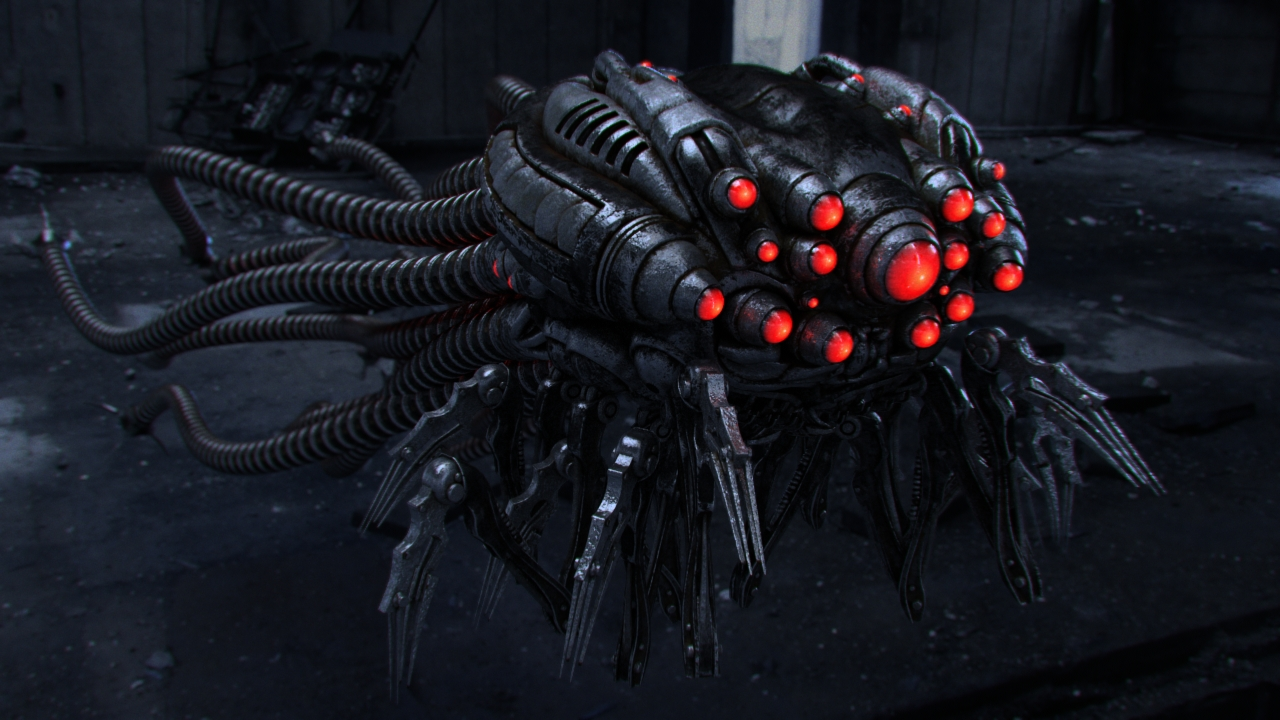
\includegraphics[width = 9cm]{matrix}
\end{center}
\end{frame}

\begin{frame}[fragile]{Assembly}
\begin{itemize}
\item MIPS, ARM, AVR, x86...
\end{itemize}
\begin{center}
\begin{tabular}{|l|l|}\hline
Operation & \$d = \$s + \$t;\\ \hline
Syntax & add \$d, \$s, \$t \\ \hline
Encoding & 0000 00ss ssst tttt dddd d000 0010 0000 \\ \hline
\end{tabular}
\end{center}
\end{frame}

\begin{frame}{Pop Quiz!}
\begin{itemize}
\item What makes a language \emph{imperative}? \pause
\item Is it true that all imperative languages are not functional? \pause
\item Name a scripting language. \pause
\item What makes a language \emph{object oriented}? \pause
\item What is a \emph{virtual machine}? \pause
\item What language is almost identical to Java? \pause
\item Is java the best language? \pause
\item Philosophical Question: Is there a way to \emph{compile} the following into English:\\
\begin{center}
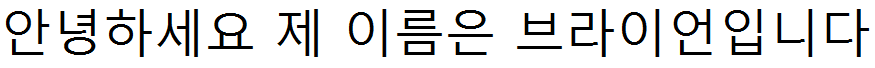
\includegraphics[width = 9cm]{korean}
\end{center}
\end{itemize}
\end{frame}

\subsection{1's and 0's, the computer's language}
\begin{frame}{1's and 0's Everywhere!}
\begin{itemize}
\item Electricity encoded as 1's and 0's are what's used by the computer. \pause
\item Computers use billions of transistors which perform boolean logic.
\item Boolean logic is just like the boolean operators we have learned (\code{\texttt{\&\&, ||, !}}), except ``1" is true and ``0" is false. \pause
\item Using AND, OR, and NOT computers do everything you see on a daily basis.
\item This means that colors, sounds, movies, everything can be represented by bits! \pause
\end{itemize}
\end{frame}

\begin{frame}{But how do we read them?}
\begin{itemize}
\item Bits can represent integers (\code{\texttt{int}}).
\item To convert a binary number to an integer we must multiply each binary number by 2 to the power of its position ($2^p$), and then add them together.
\end{itemize}
\begin{center}
\begin{tabular}{|r|c|c|c|c|c|c|}\hline
Binary & 0 & 1 & 0 & 1 & 1 & 0\\\hline \pause
Position & 5 & 4 & 3 & 2 & 1 & 0\\\hline \pause
$2^p$& $2^5$ & $2^4$ & $2^3$ & $2^2$ & $2^1$ & $2^0$\\\hline \pause
Multiplied&0\textsuperscript{*}32 &1\textsuperscript{*}16&0\textsuperscript{*}8&1\textsuperscript{*}4&1\textsuperscript{*}2&0\textsuperscript{*}1\\\hline
\end{tabular}\\\pause


Total = $0 + 16 + 0 + 4 + 2 + 0 = 22$ \\ \pause

010110 base 2 = 22 base 10
\end{center}
\end{frame}


\begin{frame}{A few more examples}
\begin{center}
\begin{tabular}{|r|c|c|c|c|}\hline
Binary & 1 & 0 & 0 & 1\\\hline \pause
Position & 3 & 2 & 1 & 0\\\hline \pause
$2^p$& $2^3$ & $2^2$ & $2^1$ & $2^0$\\\hline \pause
Multiplied&1\textsuperscript{*}8&0\textsuperscript{*}4&0\textsuperscript{*}2&1\textsuperscript{*}1\\\hline
\end{tabular}\\ \pause
Total = $8 + 0 + 0 + 1 = 9$ \\ \pause

1001 base 2 = 9 base 10

\begin{tabular}{|r|c|c|c|c|c|c|}\hline
Binary & 1 & 0 & 0 & 1 & 1 & 1\\\hline \pause
Position & 5 & 4 & 3 & 2 & 1 & 0\\\hline \pause
$2^p$& $2^5$ & $2^4$ & $2^3$ & $2^2$ & $2^1$ & $2^0$\\\hline \pause
Multiplied&1\textsuperscript{*}32 &0\textsuperscript{*}16&0\textsuperscript{*}8&1\textsuperscript{*}4&1\textsuperscript{*}2&1\textsuperscript{*}1\\\hline
\end{tabular}\pause\\
Total = $32 + 0 + 0 + 4 + 2 + 1 = 39$ \\ \pause

100111 base 2 = 39 base 10
\end{center}
\end{frame}


\begin{frame}{Converting from Integers to Binary}
\begin{center}
To go backwards we need to find the highest power of $2$ that is less than our number. This will be a `1'. We then subtract the highest power of 2 from our number, and then repeat.
\vspace{.5cm}

\uncover<1-4>{13 base 10 = ?\\}

\uncover<5>{13 base 10 = 1011 base 2\\}

\begin{tabular}{|r|c|c|c|c|}\hline
Position & 3 & 2 & 1 & 0\\\hline \pause
Multiplied&
\uncover<2->{1\textsuperscript{*}8}\only<1>{?\textsuperscript{*}8}&
\uncover<3->{0\textsuperscript{*}4}\only<2>{?\textsuperscript{*}4}&
\uncover<4->{1\textsuperscript{*}2}\only<3>{?\textsuperscript{*}2}&
\uncover<5->{1\textsuperscript{*}1}\only<4>{?\textsuperscript{*}1}\\\hline \pause
Binary &
\uncover<2->{1}\only<1>{?}&
\uncover<3->{1}\only<2>{?}&
\uncover<4->{0}\only<3>{?}&
\uncover<5->{1}\only<4>{?}\\\hline
\end{tabular}
\end{center}
\end{frame}

\begin{frame}{Quiz: One with the Machines!}
\begin{itemize}
\item 15 base 10 = \pause 1111 base 2
\item 8 base 10 = \pause 1000 base 2
\item 5 base 10 = \pause 101 base 2
\item 42 base 10 = \pause 101010 base 2
\item 11 base 2 = \pause 3 base 10
\item 010 base 2 = \pause 2 base 10
\item 1011 base 2 = \pause 11 base 10
\item 01100 base 2 = \pause 12 base 10
\item 1011011 base 10 = \pause 91 base 10
\end{itemize}
\end{frame}

\section{Bonus}
\subsection{}
\begin{frame}{Game Engine Activites!}
\begin{center}
Lets make a maze game together! If you have not done so already, download the game engine (resources) from my website.
\end{center}
\end{frame}


